\chapter{Билет №???}

\section*{Single \& Sequence}

\section{Воспоминания о \\ Sequence file}

Интерфейс sequence file позволяет передавать данные \textbf{только из kernel в user}.

Почему нет передачи из user в kernel через интерфейс sequence file?

Потому что \textbf{в ядре информации больше} (ещё больше, чем в ф.с. proc), поэтому задача передачи данных из kernel в user считается более важной.

Смысл передачи данных из kernel в user заключается в том, что информация сначала записывается в буфер ядра, и уже из буфера передается в user mode или буфер режима пользователя.
\begin{lstlisting}[language=C, label=lst:1, caption= Структуры]
struct seq_operations;

struct seq_file {
 char *buf;
 size_t size;
 size_t from;
 size_t count;
 ...
 loff_t index;
 loff_t read_pos;
 struct mutex lock;
 const struct seq_operations *op;
 int poll_event;
 const struct file *file;
 void *private;
};

struct seq_operations {
 void * (*start) (struct seq_file *m, loff_t *pos);
 void (*stop) (struct seq_file *m, void *v);
 void * (*next) (struct seq_file *m, void *v, loff_t *pos);
 int (*show) (struct seq_file *m, void *v);
};
\end{lstlisting}

Функция show выполняет все действия по передаче данных. 

start() -- начало передачи данных. Указатель pos может быть инициализирован нулем. (начало последовательности передаваемых данных);

next() -- увеличение указателя pos;

stop() -- освобождение памяти.

\begin{table}[h!]
  \centering
  \begin{tabular}{p{1\linewidth}}
    \centering
    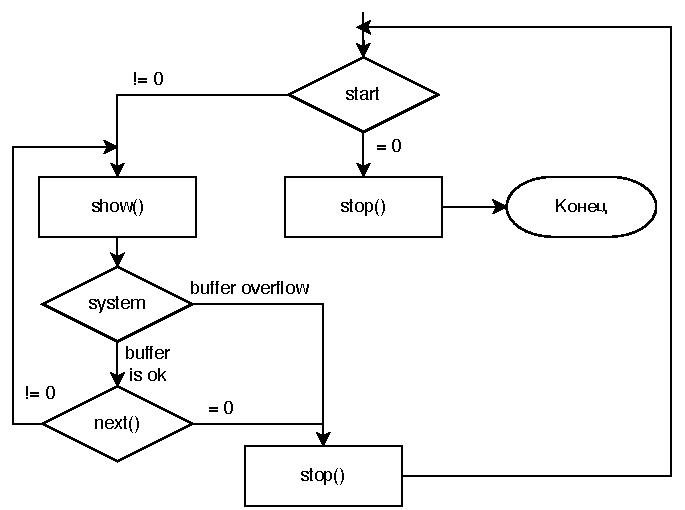
\includegraphics[width=0.95\linewidth]{./images/seq.pdf}
  \end{tabular}
\end{table}

\begin{quote}
	\textit{Это не нужно писать, чисто коммент}

	\textit{Все это добро вызывается при вызове seq\_read. То есть не нужно определять функцию чтения, нужно определить итераторы, и использовать seq\_read, которая внутри вызывает эти итераторы.}
	
	\textit{Почему 2 раза может вызываться read()? Потому что при чтении файла мы вызываем read() до тех пор, пока он не вернет 0. Соответственно, первый read() читает данные, второй возвращает 0 --- признак окончания файла.}
\end{quote}

\begin{quote}
buffer overflow --- буфер заполнен и следующая запись не может быть выполнена (переполнена может быть только помойка).

Варианты решения проблемы:
\begin{enumerate}
\item Система может создать дополнительный буфер (размер равен исходному)
\item Если память выделить невозможно, система может вернуть ошибку
\end{enumerate}
\end{quote}

\subsection{Вызов функции stop()}

Функция stop() вызывается в 3 контекстах:
\begin{enumerate}
\item сразу после start()  -- окончание вывода данных;
\item после show() -- буфер заполнен и может быть создан дополнительный объем памяти (исходный буфер может быть расширен на тот же объем, который запрашивался до этого). Если памяти нет, будет возвращена ошибка (требуется проверка);
\item после next(), когда закончились данные для вывода (нужно либо завершить работу, либо перейти на вывод другого массива данных).
\end{enumerate}

\section{Интерфейс single file}

Single file интерфейс создан для облегчения написания кода, предназначенного для передачи информации из kernel в user.

Почему single называют упрощенным? Потому что нужно определить только функцию \texttt{show}, а \texttt{start}, \texttt{stop}, \texttt{next} определять не нужно. Инициализация эих функций происходит в \texttt{single\_open}.

Single file subsystem позволяет передавать до 64 Кб. Это ограничение только для буфера передачи из kernel в user, так как обратная передача не реализована.

open --- главная точка входа.

open -> show -> seq\_printf.

\begin{quote}
Single file subsystem является промежуточным слоем отказоустойчивости за счет снижения сложности обмена данными между пространством ядра и пространством пользователя "до чего-то подобного функции printf()".
\end{quote}
\textbf{proc\_show() и proc\_my\_open()}

\begin{lstlisting}
#include <linux/module.h>
#include <linux/proc_ds.h>
#include <linux/seq_file.h>

#define PROC_FILE_NAME "myfile"

static struct proc_dir_entry *proc_file;
static char *str;

static int proc_show(struct seq_file *m, void *v)
{
  int error = 0;
  error = seq_printf(m, "%s\n", str);
  return error;
}

static int proc_my_open(struct inode *inode, struct file *file)
{
  return single_open(file, proc_show, NULL); // функция интерфейса single file
}
\end{lstlisting}

\textbf{proc\_ops}

\begin{lstlisting}
static const struct proc_ops proc_fops =
{
  // Ниже предписанные функции соответствующего интерфейса
  .proc_open = proc_my_open,
  .proc_release = single_release,
  .proc_read = seq_read
}
\end{lstlisting}

\textbf{Определение функции single\_open()}

\begin{lstlisting}
int single_open(struct file *file, int (*show)(struct seq_file *, void *), void *data)
{
  struct seq_operation *op = kmalloc(sizeof(*op), GFP_KERNEL);
  intres = -ENOMEM;
  if (op)
  {
    op->start = single_start; // функции итератора
    op->stop = single_stop;
    op->next = single_next;
    op->show = show;
    if (!res) ((struct seq_file *)file->private_data)->private = data;
    else kfree(op);
  }
  return res;
}
EXPORT_SYMBOL(single_open);
\end{lstlisting}

\section{Воспоминания о записи в файл}
Чтобы иметь возможность передавать данные из user в kernel, необходимо написать функцию write, из которой вызывать copy\_from\_user.

\section{Пример на SEQFILE (из семинара, лучше не писать, а указать норм пример из лабы)}

\begin{lstlisting}
// TODO: добавить пример на SEQFILE
static int ct_seq_show(struct seq_file *s, void *v)
{
    printk(KERN_INFO "In show() event = %d\n", *(int*)v);
    seq_printf(s, "The current value of the event number is %d\n", *(int*)v);
    return 0;
}

static void *ct_seq_start(struct seq_file *s, loff_t *pos)
{
    printk(KERN_INFO "Enter start(), pos = %ld, seq_file pos = %lu\n", *pos, s->count);
    if (pos >= limit)
    {
        printk(KERN_INFO "Done\n");
        return 0;
    }
    ...
}

// start() - начало передачи данных
// указатель pos может быть инициализирован 0 (начало последовательности передаваемых данных)
// show() - передача данных
// next() - увеличение указателя pos

// Упрощенный вариант
static void *ct_seq_next(struct seq_file *s, void *v, loff_t *pos)
{
    printk(KERN_INFO "next()\n"); // ...
    (*pos)++; // Увеличение указателя
    ...
}

// Основная задача stop() - освобождение памяти
// В stop() не может быть вызвана функция seq_printf, но может быть вызвана printk()
                   
static struct seq_operations ct_seq_ops = {
    .start = ct_seq_start,
    .next = ct_seq_next,
    .stop = ct_seq_stop,
    .show = ct_seq_show,
};

static int ct_open(struct inode *inode, struct file *file)
{
    return seq_open(file, &ct_seq_ops);
}

static struct proc_ops proc_fops = {
    .proc_open = ct_open,
    .proc_read = seq_read,
    .proc_lseek = seq_seek,
    .proc_release = seq_release, // Функции библиотеки seqfile
};
\end{lstlisting}

\section{Пример на  \\ SINGLEFILE}

\begin{lstlisting}
#include <linux/module.h>
#include <linux/kernel.h>
#include <linux/proc_fs.h>
#include <linux/seq_file.h>
#include <linux/string.h>
#include <linux/vmalloc.h>
//#include <asm/uaccess.h>

MODULE_LICENSE("GPL");
MODULE_AUTHOR("Karpova Ekaterina");

#define DIRNAME "seqfiles"
#define FILENAME "seqfile"
#define SYMLINK "seqfile_link"
#define FILEPATH DIRNAME "/" FILENAME

#define BUF_SIZE PAGE_SIZE

static struct proc_dir_entry *fortune_file = NULL;
static struct proc_dir_entry *fortune_dir = NULL;
static struct proc_dir_entry *fortune_link = NULL;

static char *cookie_buffer = NULL;  
static int write_index = 0;  
static int read_index = 0;  

static char tmp[BUF_SIZE];

ssize_t write(struct file *file, const char __user *buf, size_t len, loff_t *offp) 
{
	printk(KERN_INFO "+ seqfile: called write");
	if(len > BUF_SIZE - write_index + 1) 
	{
		printk(KERN_ERR "+ seqfile: cookie_buffer overflow");
		return -ENOSPC;
	}
	if(copy_from_user(&cookie_buffer[write_index], buf, len)) 
	{
		printk(KERN_ERR "+ seqfile: copy from user error");
		return -EFAULT;
	}
	write_index += len;
	cookie_buffer[write_index-1] = '\0';
	return len;
}

static int seqfile_show(struct seq_file *m, void *v) 
{
	printk(KERN_INFO "+ seqfile: called show");
	//if (read_index >= write_index)
		//return 0;

	int len = snprintf(tmp, BUF_SIZE, "%s\n", &cookie_buffer[read_index]);
	seq_printf(m, "%s", tmp);
	read_index += len;
	return 0;
} 

ssize_t seqfile_read(struct file *file, char __user *buf, size_t count, loff_t *offp) 
{
	printk(KERN_INFO "+ seqfile: called read");
	return seq_read(file, buf, count, offp);
}

int seqfile_open(struct inode *inode, struct file *file) 
{
	printk(KERN_INFO "+ seqfile: called open");
	return single_open(file, seqfile_show, NULL);
}

int seqfile_release(struct inode *inode, struct file *file) 
{
	printk(KERN_INFO "+ seqfile: called release");
	return single_release(inode, file);
}

static struct proc_ops fops = {
	.proc_open = seqfile_open,
	.proc_read = seqfile_read,
	.proc_write = write,
	.proc_release = seqfile_release, 
};

void freemem(void) 
{
	if (cookie_buffer)
		vfree(cookie_buffer);
	if (fortune_link)
		remove_proc_entry(SYMLINK, NULL);
	if (fortune_file)
		remove_proc_entry(FILENAME, fortune_dir);
	if (fortune_dir)
		remove_proc_entry(DIRNAME, NULL);
}

static int __init init_seqfile_module(void) 
{	
	if (!(cookie_buffer = vmalloc(BUF_SIZE))) 
	{
		freemem();
		printk(KERN_ERR "+ seqfile: error during vmalloc");
		return -ENOMEM;
	}
	memset(cookie_buffer, 0, BUF_SIZE);
	if (!(fortune_dir = proc_mkdir(DIRNAME, NULL))) 
	{
		freemem();
		printk(KERN_ERR "+ seqfile: error during directory creation");
		return -ENOMEM;
	} 
	else if (!(fortune_file = proc_create(FILENAME, 0666, fortune_dir, &fops))) 
	{
		freemem();
		printk(KERN_ERR "+ seqfile: error during file creation");
		return -ENOMEM;
	} 
	else if (!(fortune_link = proc_symlink(SYMLINK, NULL, FILEPATH))) 
	{
		freemem();
		printk(KERN_ERR "+ seqfile: error during symlink creation");
		return -ENOMEM;
	}
	write_index = 0;
	read_index = 0;
	printk(KERN_INFO "+ module loaded");
	return 0;
}

static void __exit exit_seqfile_module(void) 
{
	freemem();
	printk(KERN_INFO "+ seqfile: unloaded");
}

module_init(init_seqfile_module);
module_exit(exit_seqfile_module);

\end{lstlisting}

\section{Пример на SEQFILE}

\begin{lstlisting}
#include <linux/module.h>
#include <linux/kernel.h>
#include <linux/proc_fs.h>
#include <linux/seq_file.h>
#include <linux/string.h>
#include <linux/vmalloc.h>

MODULE_LICENSE("GPL");
MODULE_AUTHOR("Aleksey Knyazhev");

#define DIRNAME "seqfiles"
#define FILENAME "seqfile"
#define SYMLINK "seqfile_link"
#define FILEPATH DIRNAME "/" FILENAME

#define BUF_SIZE PAGE_SIZE

static struct proc_dir_entry *seqfile_file = NULL;
static struct proc_dir_entry *seqfile_dir = NULL;
static struct proc_dir_entry *seqfile_link = NULL;

static char *cookie_buffer = NULL;  
static int index = 0;  

ssize_t custom_write(struct file *file, const char __user *buf, size_t len, loff_t *offp) 
{
 printk(KERN_INFO "+ seqfile: called write");
 if(len > BUF_SIZE - index + 1) 
 {
  printk(KERN_ERR "+ seqfile: cookie_buffer overflow");
  return -ENOSPC;
 }
 if(copy_from_user(&cookie_buffer[index], buf, len)) 
 {
  printk(KERN_ERR "+ seqfile: copy from user error");
  return -EFAULT;
 }
 index += len;
 cookie_buffer[index-1] = '\n';
 return len;
}

static int seqfile_show(struct seq_file *m, void *v) 
{
 printk(KERN_INFO "+ seqfile: called show");
 seq_printf(m, "%s", cookie_buffer);
 return 0;
} 

ssize_t seqfile_read(struct file *file, char __user *buf, size_t count, loff_t *offp) 
{
 printk(KERN_INFO "+ seqfile: called read");
 return seq_read(file, buf, count, offp);
}

int seqfile_open(struct inode *inode, struct file *file) 
{
 printk(KERN_INFO "+ seqfile: called open");
 return single_open(file, seqfile_show, NULL);
}

int seqfile_release(struct inode *inode, struct file *file) 
{
 printk(KERN_INFO "+ seqfile: called release");
 return single_release(inode, file);
}

static struct proc_ops fops = {
 .proc_open = seqfile_open,
 .proc_read = seqfile_read,
 .proc_write = custom_write,
 .proc_release = seqfile_release, 
};

void freemem(void) 
{
 if (cookie_buffer)
  vfree(cookie_buffer);
 if (seqfile_link)
  remove_proc_entry(SYMLINK, NULL);
 if (seqfile_file)
  remove_proc_entry(FILENAME, seqfile_dir);
 if (seqfile_dir)
  remove_proc_entry(DIRNAME, NULL);
}

static int __init init_seqfile_module(void) 
{ 
 if (!(cookie_buffer = vmalloc(BUF_SIZE))) 
 {
  freemem();
  printk(KERN_ERR "+ seqfile: error during vmalloc");
  return -ENOMEM;
 }
 memset(cookie_buffer, 0, BUF_SIZE);
 if (!(seqfile_dir = proc_mkdir(DIRNAME, NULL))) 
 {
  freemem();
  printk(KERN_ERR "+ seqfile: error during directory creation");
  return -ENOMEM;
 } 
 else if (!(seqfile_file = proc_create(FILENAME, 0666, seqfile_dir, &fops))) 
 {
  freemem();
  printk(KERN_ERR "+ seqfile: error during file creation");
  return -ENOMEM;
 } 
 else if (!(seqfile_link = proc_symlink(SYMLINK, NULL, FILEPATH))) 
 {
  freemem();
  printk(KERN_ERR "+ seqfile: error during symlink creation");
  return -ENOMEM;
 }
 index = 0;
 printk(KERN_INFO "+ module loaded");
 return 0;
}

static void __exit exit_seqfile_module(void) 
{
 freemem();
 printk(KERN_INFO "+ seqfile: unloaded");
}

module_init(init_seqfile_module);
module_exit(exit_seqfile_module);
\end{lstlisting}


